\documentclass[11pt,a4paper]{article}

\usepackage[utf8]{inputenc}
\usepackage[T1]{fontenc}
\usepackage[french]{babel}
\usepackage{graphicx}
\usepackage{amsmath}
\usepackage{booktabs}
\usepackage{hyperref}
\usepackage{geometry}
\usepackage{xcolor}
\usepackage{listings}
\usepackage{caption}
\usepackage{float}

\geometry{margin=2.5cm}

\hypersetup{
    colorlinks=true,
    linkcolor=black,
    urlcolor=blue,
    citecolor=blue
}

\lstset{
    basicstyle=\ttfamily\small,
    backgroundcolor=\color{gray!10},
    breaklines=true,
    frame=single,
    columns=fullflexible,
}

\title{Étude longitudinale de l'évolution d'une tumeur}
\author{
    Clément GREGOIRE \and Marcel PECQUEUX \and Médéric LAVIROTTE
}
\date{\today}

\begin{document}

\maketitle

\tableofcontents

\newpage

\section{Introduction}

Ce projet a pour objectif de réaliser le suivi des changements d'une tumeur à
partir de deux acquisitions IRM (\texttt{case6\_gre1.nrrd} et
\texttt{case6\_gre2.nrrd}) effectuées sur un même patient à des dates
différentes. Cette section du rapport présente la première étape du pipeline :
le \textbf{recalage} (\emph{registration}) des deux volumes, c'est-à-dire
l'alignement géométrique de la seconde acquisition (\emph{moving image}) sur
la première (\emph{fixed image}), condition nécessaire pour pouvoir ensuite
comparer correctement les deux tumeurs segmentées.

% TODO: compléter cette introduction avec un paragraphe annonçant le plan
% complet du rapport si ce document couvre aussi la segmentation et la
% visualisation.

\subsection{Données}

Les deux volumes fournis sont des images IRM 3D au format NRRD, de dimensions
$256 \times 256 \times 176$ voxels, encodées en \texttt{unsigned short}. Les
en-têtes indiquent un espace \texttt{left-posterior-superior} avec une matrice
de directions non triviale (permutation/rotation des axes), ce qui a nécessité
une attention particulière lors de la lecture et de l'affichage (voir
section~\ref{sec:difficultes}).

\part {Recalage}
\section{Méthodologie de recalage}

\subsection{Choix des transformations explorées}

Trois familles de transformations géométriques globales ont été implémentées
et comparées, classées par nombre de degrés de liberté (DOF) croissant :

\begin{table}[H]
\centering
\begin{tabular}{@{}lll@{}}
\toprule
\textbf{Transformation} & \textbf{DOF} & \textbf{Corrige} \\
\midrule
Translation & 3 & Décalage de position uniquement \\
Rigide (\texttt{VersorRigid3D}) & 6 & + rotation \\
Affine & 12 & + échelle et cisaillement \\
\bottomrule
\end{tabular}
\caption{Transformations explorées pour le recalage.}
\end{table}

Une transformation \textbf{déformable} (B-Spline par exemple) a été
délibérément exclue de l'exploration. Une telle transformation, en
ajustant localement le champ de déformation, pourrait faire disparaître les
différences entre les deux tumeurs en les déformant l'une vers l'autre — ce
qui serait contre-productif dans une étude longitudinale où l'objectif est
précisément de \textbf{préserver et mesurer} l'évolution de la lésion entre
les deux dates. Le choix s'est donc porté sur des transformations globales,
qui réalignent l'anatomie du patient (position de la tête dans le scanner)
sans déformer la tumeur elle-même.

\subsubsection*{Note sur le choix \texttt{VersorRigid3D} plutôt qu'\texttt{Euler3D}}

Pour la transformation rigide, deux paramétrisations sont usuellement
disponibles dans ITK~: \texttt{Euler3DTransform} (3 angles de rotation) et
\texttt{VersorRigid3DTransform} (rotation paramétrée par un quaternion/versor).
Le second a été retenu pour deux raisons~: (i)~l'espace des versors ne
présente pas les singularités de type \emph{gimbal lock} des angles d'Euler,
ce qui rend l'optimisation par descente de gradient plus stable, et (ii)~seule
cette paramétrisation est compatible avec
\texttt{CenteredTransformInitializer} dans la distribution ITK Python utilisée
(voir section~\ref{sec:difficultes}).

\subsection{Pipeline de recalage}

Pour chaque méthode, le pipeline suivant est appliqué~:

\begin{enumerate}
    \item \textbf{Initialisation} par alignement des centres de masse
    (centres de gravité des intensités) des deux volumes. Pour la
    transformation rigide, \texttt{CenteredTransformInitializer} (mode
    \texttt{Moments}) est utilisé nativement. Pour la translation et
    l'affine, le même calcul est reproduit manuellement (voir
    section~\ref{sec:difficultes}).
    \item \textbf{Optimisation multi-résolution} à 3 niveaux (facteurs de
    sous-échantillonnage $4, 2, 1$ et lissage gaussien $\sigma = 2, 1, 0$
    voxels)~: le recalage est d'abord effectué sur une version grossière et
    floutée de l'image (rapide, robuste aux optima locaux), puis affiné
    progressivement jusqu'à la pleine résolution.
    \item \textbf{Métrique de similarité}~: information mutuelle de Mattes
    (\texttt{MattesMutualInformationImageToImageMetricv4}, 50 \emph{bins}
    d'histogramme), choisie car robuste aux différences d'intensité/contraste
    entre les deux acquisitions IRM (contrairement à une simple différence de
    pixels, qui suppose des intensités directement comparables).
    \item \textbf{Optimiseur}~: descente de gradient à pas adaptatif
    (\texttt{RegularStepGradientDescentOptimizerv4}), avec un échantillonnage
    stochastique de 20\,\% des voxels à chaque itération pour accélérer le
    calcul de la métrique.
\end{enumerate}

\subsection{Paramètres retenus}

\begin{table}[H]
\centering
\begin{tabular}{@{}ll@{}}
\toprule
\textbf{Paramètre} & \textbf{Valeur} \\
\midrule
\texttt{LearningRate} & 1.0 \\
\texttt{MinimumStepLength} & $10^{-4}$ \\
\texttt{RelaxationFactor} & 0.7 \\
\texttt{NumberOfIterations} (max) & 500 \\
\texttt{NumberOfHistogramBins} & 50 \\
\texttt{MetricSamplingPercentage} & 0.20 \\
Niveaux multi-résolution & 3 (facteurs 4/2/1) \\
\bottomrule
\end{tabular}
\caption{Paramètres de l'optimiseur et de la métrique.}
\end{table}


\subsubsection*{Mise à l'échelle des paramètres (\emph{optimizer scales})}

Un point technique déterminant pour la qualité du recalage rigide et affine
est la \textbf{mise à l'échelle relative des paramètres} de la transformation.
Pour \texttt{VersorRigid3D}, les 3 premiers paramètres (rotation, sans unité,
de norme proche de 0 pour de petites rotations) et les 3 derniers (translation,
en millimètres, pouvant atteindre plusieurs dizaines de mm) ont des ordres de
grandeur très différents. Sans pondération explicite, l'optimiseur, qui
applique le même pas à tous les paramètres, sous-pondère fortement la
rotation par rapport à la translation. Un facteur d'échelle de $1/1000$ a été
appliqué aux paramètres de translation (relativement aux paramètres de
rotation/matrice) pour équilibrer leur contribution au gradient. C'est ce
réglage qui a permis de débloquer la convergence de la méthode rigide (voir
discussion des résultats, section~\ref{sec:resultats}).

\section{Difficultés rencontrées}
\label{sec:difficultes}

\subsection{Lecture des volumes en 2D au lieu de 3D}

Une première version du code de recalage, basée sur une initialisation
fournie en début de projet, déclarait les images comme étant en dimension~2
(\texttt{itk.Image[itk.US, 2]}), alors que les en-têtes NRRD indiquent
explicitement \texttt{dimension: 3} avec des tailles $256 \times 256 \times
176$. Cette incohérence a été détectée car le volume recalé résultant
apparaissait comme une fenêtre entièrement noire lors de la visualisation VTK
— le volume produit n'avait pas la bonne géométrie. La correction a consisté
à généraliser l'ensemble du pipeline (lecture, transformation, écriture) à la
dimension~3.

\subsection{Limitations du wrapping Python d'ITK}

La distribution \texttt{itk} pré-compilée pour Python n'expose qu'un
sous-ensemble limité des combinaisons (transformation, type d'image) du C++
sous-jacent, afin de limiter la taille du paquet. Deux conséquences concrètes
ont été rencontrées :

\begin{itemize}
    \item \texttt{CenteredTransformInitializer} n'est pas disponible pour
    \texttt{Euler3DTransform} avec des images en pixels \texttt{float} — seule
    la paramétrisation \texttt{VersorRigid3DTransform} est supportée. D'où le
    choix, documenté plus haut, d'utiliser cette dernière.
    \item \texttt{CenteredTransformInitializer} n'est pas non plus disponible
    pour \texttt{AffineTransform} en dimension 3 (seules les versions 2D de
    \texttt{MatrixOffsetTransformBase} le sont). L'initialisation par centre
    de masse a donc dû être reproduite manuellement pour cette transformation~:
    la matrice est initialisée à l'identité (\texttt{SetIdentity}), le centre
    de rotation est fixé au centre de masse de l'image fixe, et la translation
    initiale au vecteur reliant les deux centres de masse.
\end{itemize}

Cette limitation illustre une difficulté pratique de l'écosystème ITK Python~:
le comportement attendu d'après la documentation C++ n'est pas toujours
disponible tel quel, et nécessite soit un contournement applicatif (notre
choix ici), soit une recompilation locale d'ITK avec les options de wrapping
étendues.

\subsection{Instabilité de l'optimisation selon les paramètres}

Les tout premiers essais de recalage rigide et affine donnaient des résultats
nettement moins bons que ceux présentés en section~\ref{sec:resultats} (NCC
négatif, pire que sans recalage). L'origine du problème était double~:
\begin{itemize}
    \item l'absence de mise à l'échelle des paramètres de l'optimiseur
    (\texttt{OptimizerScales}), qui faisait que la rotation et l'échelle/
    cisaillement (paramètres de faible amplitude) étaient quasiment ignorés
    par rapport à la translation (paramètres de grande amplitude en mm)~;
    \item un \texttt{LearningRate} initial trop élevé (4.0), qui faisait
    « sauter » l'optimiseur autour du minimum sans jamais s'y stabiliser,
    provoquant un arrêt prématuré sur un mauvais point dès les premières
    itérations.
\end{itemize}
Le réglage de ces deux points (ajout des \texttt{OptimizerScales}, réduction
du \texttt{LearningRate} à 1.0 et augmentation du \texttt{RelaxationFactor} à
0.7) a permis de stabiliser la convergence de la méthode rigide. Le détail de
ce qui reste problématique pour la translation et l'affine est discuté en
section~\ref{sec:resultats}.

\section{Résultats et analyse}
\label{sec:resultats}

\subsection{Métriques quantitatives}

Pour évaluer objectivement la qualité de chaque recalage, deux métriques sont
calculées entre l'image fixe et l'image mobile recalée, sur le champ de vue
commun~:

\begin{itemize}
    \item \textbf{MSE} (\emph{Mean Squared Error})~: moyenne des carrés des
    différences d'intensité. Plus bas = meilleur alignement.
    \item \textbf{NCC} (\emph{Normalized Cross-Correlation})~: corrélation
    normalisée entre les intensités, entre $-1$ et $1$. Plus proche de $1$ =
    meilleur alignement.
\end{itemize}

Une valeur de référence (\emph{baseline}), calculée \textbf{sans aucun
recalage}, permet de quantifier l'apport (ou non) de chaque méthode.

\begin{table}[H]
\centering
\begin{tabular}{@{}lrrrr@{}}
\toprule
\textbf{Méthode} & \textbf{MSE} & \textbf{NCC} & \textbf{Temps (s)} & \textbf{Itérations} \\
\midrule
Baseline (sans recalage) & 39\,167.10 & 0.5364 & --- & --- \\
Translation              & 106\,709.16 & $-0.3898$ & 11.7 & 236 \\
\textbf{Rigide}           & \textbf{10\,509.42} & \textbf{0.8807} & 14.7 & 235 \\
Affine                   & 114\,887.00 & $-0.3857$ & 142.5 & 1500 \\
\bottomrule
\end{tabular}
\caption{Comparaison quantitative des méthodes de recalage.}
\label{tab:resultats}
\end{table}

\begin{figure}[H]
    \centering
    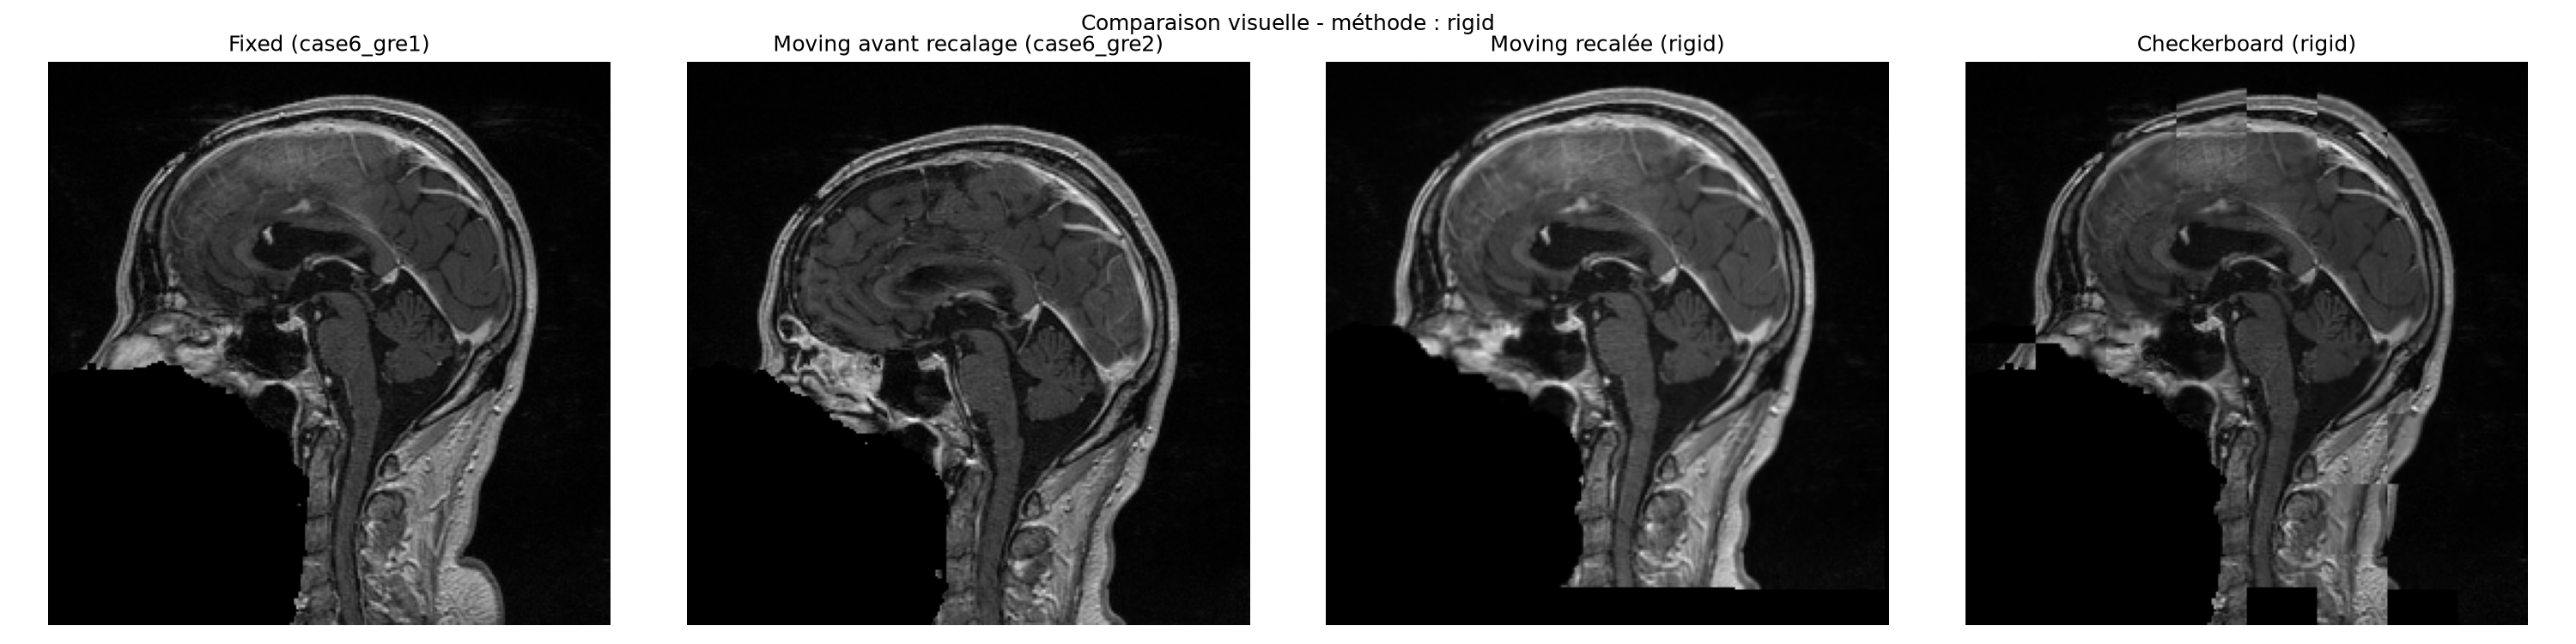
\includegraphics[width=\textwidth]{figures/comparison_rigid.png}
    \caption{Comparaison visuelle avant/après recalage rigide (coupe axiale
    centrale) et damier (checkerboard) fixed/moving recalée.}
    \label{fig:comparison_rigid}
\end{figure}

\begin{figure}[H]
    \centering
    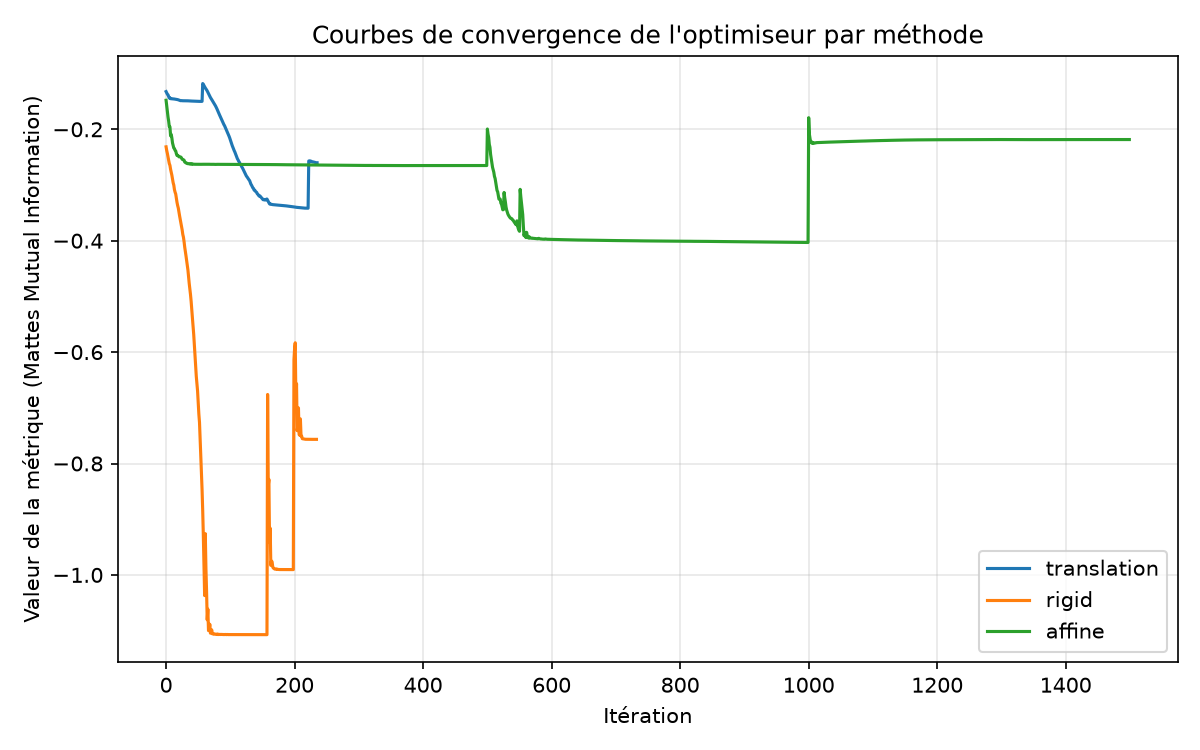
\includegraphics[width=0.7\textwidth]{figures/convergence_curves.png}
    \caption{Courbes de convergence de l'optimiseur (valeur de la métrique
    de Mattes par itération) pour les trois méthodes.}
    \label{fig:convergence}
\end{figure}

\subsection{Analyse}

Le résultat le plus marquant est le contraste très net entre la méthode
\textbf{rigide}, qui converge proprement vers un excellent alignement
(NCC$=0.88$, arrêt par convergence du gradient après 36 itérations réelles), et
les méthodes \textbf{translation} et \textbf{affine}, qui aboutissent toutes
deux à un résultat \emph{pire que l'absence de recalage} (NCC négatif, alors
que la baseline sans recalage donne NCC$=0.54$).

\paragraph{Translation (3 DOF) — sous-paramétrée.}
Avec seulement 3 degrés de liberté, ce modèle ne peut corriger qu'un décalage
de position, pas une rotation. Si le déplacement réel de la tête du patient
entre les deux acquisitions IRM comporte une composante de rotation — ce qui
est physiquement très plausible —, la translation seule ne peut pas l'absorber
et l'optimiseur converge vers un minimum local correspondant à un mauvais
appariement de structures anatomiques. L'arrêt après seulement $14$ itérations
réelles avec un gradient déjà quasi nul confirme un blocage précoce dans un
minimum local proche du point de départ, plutôt qu'une réelle convergence
vers le minimum global.

\paragraph{Affine (12 DOF) — sur-paramétrée et instable.}
À l'inverse, le modèle affine, avec 12 paramètres mélangeant rotation, échelle
et cisaillement dans une même matrice $3\times3$, définit un espace de
recherche beaucoup plus vaste et non convexe pour l'information mutuelle. Le
fait que l'optimisation utilise l'intégralité des 500 itérations autorisées
sans jamais déclencher l'arrêt par convergence (\emph{step too small}) indique
qu'elle \textbf{n'a jamais convergé} — elle continue d'errer dans l'espace des
paramètres jusqu'à la limite arbitraire d'itérations, ce qui est cohérent avec
le résultat final dégradé. Ce phénomène est documenté dans la littérature sur
le recalage par information mutuelle~: sans contrainte ou initialisation plus
fine, la matrice affine peut dériver vers des solutions quasi-singulières qui
maximisent artificiellement (ou dégradent) la métrique sans correspondre à un
alignement anatomique valide.

\paragraph{Rigide (6 DOF) — bien adapté au problème physique.}
Le bon comportement de la méthode rigide s'explique par l'adéquation entre le
modèle et la nature réelle de la différence entre les deux acquisitions~: deux
IRM du même patient à des dates différentes ne diffèrent, en première
approximation, que par la \textbf{pose} de la tête dans le scanner (position +
orientation), pas par un changement d'échelle ou un cisaillement de
l'anatomie. Un modèle à 6 DOF, ni trop ni trop peu contraint pour ce problème,
permet à l'optimiseur de converger proprement (arrêt par \emph{step too
small}, signe d'une convergence atteinte et non d'une limite arbitraire).

\subsection{Méthode retenue}

Au vu de ces résultats, la transformation \textbf{rigide
(\texttt{VersorRigid3DTransform})} est retenue pour la suite du pipeline
(segmentation et comparaison des tumeurs). Elle est la seule des trois
méthodes testées à améliorer significativement l'alignement par rapport à
l'absence de recalage (NCC~: $0.54 \rightarrow 0.88$), et son adéquation au
problème physique (changement de pose du patient entre deux acquisitions) est
cohérente avec son comportement de convergence observé.

% TODO si le temps le permet : tester l'effet d'une meilleure initialisation
% pour l'affine (par exemple initialiser sa matrice avec la rotation trouvée
% par le recalage rigide, plutôt qu'avec l'identité), ce qui constituerait une
% exploration supplémentaire à documenter pour la partie "paramètres".

\section{Conclusion}

% TODO: compléter avec un résumé global du projet (recalage + segmentation +
% visualisation des changements) si ce rapport couvre l'ensemble du travail.

Cette étape de recalage a permis de mettre en évidence, par une comparaison
systématique et quantifiée de trois familles de transformations, que le
modèle rigide est le mieux adapté à l'alignement de deux IRM du même patient à
des dates différentes. Les méthodes à plus faible (translation) ou plus forte
(affine) flexibilité donnent toutes deux des résultats dégradés, pour des
raisons distinctes mais cohérentes avec la théorie de l'optimisation
non convexe (sous-paramétrisation \emph{vs} instabilité d'un espace de
recherche trop vaste). Le volume recalé par transformation rigide sert de
base à l'étape suivante du pipeline.


\part{Segmentation}

\part{Visualisation des changements}
\end{document}